\section{Reinforcement Learning Komponenten}
In den folgenden Abschnitten werden die Komponenten beschrieben, die \acl{RL} implementieren. 
Dies umfasst die Agenten für \bothAlgs sowie deren Lerndaten in Form der Q- und \wtable.

\subsection{\qlearning und \sarsa Agenten}
Da \bothAlgs eng verwandte \ac{TDL} Algorithmen sind, wurde eine abstrakte Klasse RLTDAgent erstellt, von der die konkreten Agenten abgeleitet werden. 
Neben dem Vorteil der Redundanzvermeidung nutzen AgentQLearning und AgentSARSA ein einheitliches Interface und können in den Trainings- und Evaluationsmethoden untereinander ausgetauscht werden.

Der Unterschied der beiden Algorithmen liegt in deren Vorgehen in jedem Zeitschritt, weshalb die move-Methode als abstrakt deklariert wurde. 
\cref{listing:moveQL} und \cref{listing:movesarsa} zeigen die Implementierung der move-Methode des AgentQLearning und AgentSARSA. 
Wie in \cref{chap:vergleich} erklärt, unterscheiden sie sich in zwei Aspekten. 
Einerseits in der Aktion, die jeweils für das Update verwendet wird. 
Bei \qlearning ist dies immer Aktion mit dem höchsten  \qValue und bei \sarsa die Aktion, die der Agent wirklich durchführt. 
Andererseits liegt der Unterschied darin, dass \qlearning das \ac{TD} Update durchführt, bevor es die Aktion für den Zustand $S'$ wählt. 
Da im Fall von \acs{TTT} kein Zustandswechsel möglich ist, bei dem ein Zustand $S$ sein eigener Folgezustand $S'$ ist, könnte das \acl{TD} Update auch nach der Aktionswahl durchgeführt werden. 
Dadurch reduziert sich der Unterschied auf die Wahl der Aktion für das Update. 
Auf diese Reduktion wurde verzichtet, um die Algorithmen wie vorgestellt zu implementieren und den Unterschied deutlich im Source-Code darzustellen. Beide move-Methoden implementieren die $\epsilon$-greedy-Policy \cite[S. 27f.]{suttonReinforcementLearningIntroduction2018}.

\begin{listing}[p]
\caption{move-Methode des Agent Q-Learning}
\label{listing:moveQL}
\inputminted{java}{04_Artefakte/03_Listings/move_qlearning.java}
\end{listing}

\begin{listing}[p]
\caption{move-Methode des Agent Sarsa}
\label{listing:movesarsa}
\inputminted{java}{04_Artefakte/03_Listings/move_sarsa.java}
\end{listing}

\subsection{Lerndaten}
\begin{figure}
    \centering
    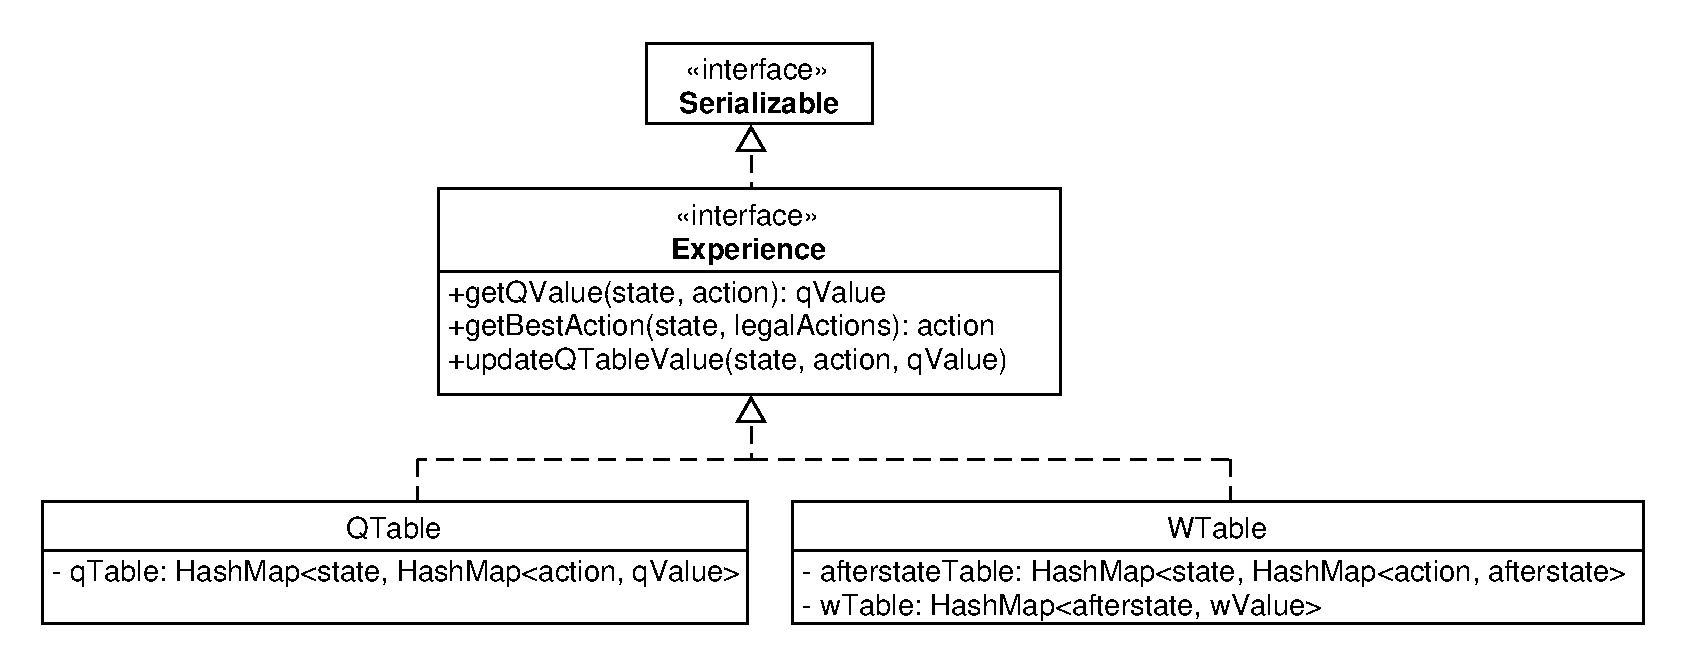
\includegraphics[width=\textwidth]{04_Artefakte/01_Abbildungen/uml/uml_experience.pdf}
    \caption{Experience Interface und implementierende Klassen}
    \label{fig:uml_experience}
\end{figure}

Die gesammelte Erfahrung des Agenten wird in der Anwendung durch das Experience Interface implementiert, das in \cref{fig:uml_experience} dargestellt ist. 
Da der Agent die Lerndaten in Form einer \qtable oder \wtable organisieren kann, bietet das Experience Interface dem Agenten einheitliche Methoden zum Zugriff auf die Lerndaten. 
Die in \cref{sec:afterstates} beschriebene Abbildung der \ac{SA Tupel} auf den resultierenden Afterstate, wird so ebenfalls vom Agenten entkoppelt und erfolgt in der Klasse WTable.

Eine Experience Instanz wird nicht durch einen Agenten selbst erzeugt, sondern im Konstruktor übergeben. 
Diese Implementierung hat zwei Gründe. 
Zum einen ist es notwendig, damit zwei Agenten im Rahmen von \splay gemeinsam eine Experience Instanz füllen können. 
Zum anderen verdeutlicht die Trennung, dass die Erfahrung kein inhärenter Bestandteil eines Agenten ist, sondern diese nur vom Agenten verwendet werden. 
Der Unterschied eines trainierten und untrainierten Agenten eines Algorithmus besteht, abgesehen von den Hyperparametern, in der Erfahrung, auf die jeweils zugegriffen wird. 
Aus diesem Grund implementiert Experience das Java Interface Serializable, wodurch Erfahrungen als Datei exportiert und importiert werden können, sodass Agenten erneut geladen werden können, um weitere Tests durchzuführen. 
In der Implementierung sind \qtable und der \afterstateTable beide mittels geschachtelten HashMaps umgesetzt, für die als Schlüssel jeweils die eindeutigen Zustände $B_{S}$ und Aktionen verwendet werden.

Im vorgestellten Pseudocode von \bothAlgs werden die \qValues aller \ac{SA Tupel} vor der ersten Episode willkürlich initialisiert. 
Dies setzt voraus, dass eine Liste aller legalen \ac{SA Tupel} vorliegt. 
Stattdessen werden in der Implementierung die \qtable und \wtable dynamisch konstruiert. 
Bei jedem Aufruf der move-Methode eines Agenten reicht dieser den aktuellen Zustand sowie die legalen Aktionen zur Initialisierung weiter. 
Dies ermöglicht die Erfassung der Zustandsanzahl, die der Agent im Rahmen des Trainings besucht hat. 
Im Konstruktor kann der initiale \qValue übergeben werden. 
In dieser Arbeit wird ausschließlich 0 verwendet. 